\chapter{Rings}\label{chap:rings}
\begin{summary}
\item Prime ideals and maximal ideals, relation to fields and integral domains. Application of quotients to constructing fields by adjunction of elements. Degree of a field extension, the tower law.
\item Euclidean domains. Principal ideal domains. EDs are PIDs. Unique factorisation for PIDs. Gauss's lemma and Eisenstein's criterion for irreducibility.
\end{summary}

\section{Rings}
\subsection{Definitions and Properties}
\begin{definition}[Ring]
A \vocab{ring}\index{ring} $R$ is a set together with two binary operations $+$ and $\times$ (called addition and multiplication), satisfying the following axioms:
\begin{enumerate}[label=(\roman*)]
\item $(R,+)$ is an abelian group, with identity $0$;
\item $\times$ is associative: $(a\times b)\times c=a\times(b\times c)$ for all $a,b,c\in R$;
\item $\times$ distributes over $+$: for all $a,b,c\in R$,
\begin{align*}
a\times(b+c)&=(a\times b)+(a\times c),\\
(a+b)\times c&=(a\times c)+(b\times c).
\end{align*}
\end{enumerate}
\end{definition}

\begin{notation}
We simply write $ab$ rather than $a\times b$, for $a,b\in R$.
\end{notation}

\begin{notation}
Denote the additive identity of $a\in R$ by $-a$.
\end{notation}

We say $R$ is \emph{commutative} if multiplication is commutative.

We say $R$ has an \emph{identity} if there exists $1\in R$ such that
\[1\times a=a\times 1=a\quad(a\in R).\]

In general, a ring may not necessarily be commutative or have multiplicative inverses; when they do, we give such rings special names.

\begin{definition}
A ring $R$ with identity $1$, where $1\neq0$, is called a \vocab{division ring}\index{division ring} if every $a\in R\setminus\{0\}$ has a multiplicative inverse, i.e., exists $b\in R$ such that $ab=ba=1$.

A commutative division ring is called a \vocab{field}\index{field}.
\end{definition}

\begin{figure}[H]
\centering
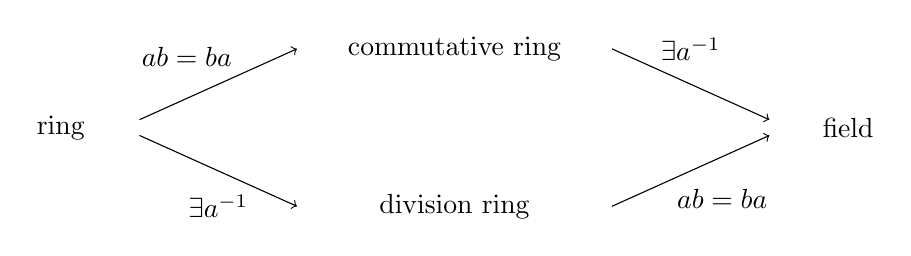
\begin{tikzpicture}
\node at (-0.5,0) {ring};
\draw[->] (0.5,0.1) -- (2.5,1);
\node at (1.1,0.9) {$ab=ba$};
\node at (4.5,1) {commutative ring};
\draw[->] (0.5,-0.1) -- (2.5,-1);
\node at (1.5,-1) {$\exists a^{-1}$};
\node at (4.5,-1) {division ring};
\draw[->] (6.5,1) -- (8.5,0.1);
\node at (7.5,1) {$\exists a^{-1}$};
\draw[->] (6.5,-1) -- (8.5,-0.1);
\node at (7.9,-0.9) {$ab=ba$};
\node at (9.5,0) {field};
\end{tikzpicture}
\end{figure}

\begin{example} \
\begin{itemize}
\item $\ZZ$ is the prototypical ring; it is not a field.
\item $\QQ$, $\RR$, $\CC$ are fields.
\item $\ZZ/n\ZZ$ is a commutative ring with identity $\bar{1}$ under addition and multiplication of residue classes.
\item $2\ZZ$ is a commutative ring without identity.
\item The trivial ring $R=\{0\}$ is a commutative ring with identity $1=0$.
\item The ring of (polynomial/continuous/differentiable) functions on $\RR$.
\item The endomorphism ring $\End_\RR(V)$ of a vector space $V$ over $\RR$ is a non-commutative ring.
\item The Hamilton Quaternions $\HH$. Historically the first example of a non-commutative ring.
\end{itemize}
\end{example}

\begin{lemma}[Basic properties]
Let $R$ be a ring.
\begin{enumerate}[label=(\roman*)]
\item $0a=a0=0$ for all $a\in R$.
\item $(-a)b=a(-b)=-(ab)$ for all $a,b\in R$.
\item $(-a)(-b)=ab$ for all $a,b\in R$.
\item If $R$ has identity $1$, then the identity is unique and $-a=(-1)a$.
\end{enumerate}
\end{lemma}

\begin{proof}
These all follow from the distributive laws and cancellation in the additive group $(R,+)$.
\begin{enumerate}[label=(\roman*)]
\item We have $0a=(0+0)a=0a+0a$. Then the cancellation law implies $0a=0$. 

Similarly, $a0=a(0+0)=a0+a0$. Thus $a0=0$.

\item We have $ab+(-a)b=\brac{a+(-a)}b=0b=0$. Thus $(-a)b=-(ab)$. 

Similarly, $ab+a(-b)=a\brac{b+(-b)}=a0=0$. Thus $a(-b)=-(ab)$.

\item Using (ii), $(-a)(-b)=-a(-b)=-\brac{-(ab)}=ab$.

\item Suppose $1$ and $1^\prime$ are identities of $R$. Then $1=1\times1^\prime=1^\prime$.

Since $(-1)a+a=(-1)a+1a=\brac{(-1)+1}a=0a=0$, it follows that $-a=(-1)a$.
\end{enumerate}
\end{proof}

\subsection{Subrings}
Having defined the notion of a ring, there is a natural notion of a subring.

\begin{definition}[Subring]
Let $R$ be a ring. We say $S\subset R$ is a \vocab{subring}\index{subring} of $R$, if $S$ is a subgroup of $R$ that is closed under multiplication.
\end{definition}

\begin{example} \
\begin{itemize}
\item $\ZZ$ is a subring of $\QQ$, and $\QQ$ is a subring of $\RR$.
\item $n\ZZ=\{nk\in\ZZ\mid k\in\ZZ\}$ is a subring of $\ZZ$.
\item The real-valued differentiable functions on $\RR$ form a subring of the ring of continuous functions.
\item $\ZZ[i]=\{x+yi\mid x,y\in\ZZ\}$ is a subring of $\CC$, called the ring of Guassian integers.
\item $\QQ[\sqrt{2}]=\{x+y\sqrt{2}\mid x,y\in\QQ\}$ is a subring of $\RR$.
\item $S=\ZZ+\ZZ i+\ZZ j+\ZZ k$ form a subring of $\HH$.
\end{itemize}
We will use the square brackets notation quite frequently. It should be clear what it should mean, and we will define it properly later.
\end{example}

If $R$ contains $1$, then $S$ is a (unital) subring if $1_R\in S$. We assume subrings are unital unless otherwise specified.

\begin{lemma}[Subring criterion]
Let $R$ be a ring, $S\subset R$. Then $S$ is a subring of $R$ if and only if
\begin{enumerate}[label=(\roman*)]
\item $1\in S$;\hfill(non-empty)
\item $ab,a-b\in S$ for all $a,b\in S$.\hfill(closed under multiplication and subtraction)
\end{enumerate}
\end{lemma}

\begin{proof} \

\fbox{$\implies$} 

\fbox{$\impliedby$} The condition that $a-b\in S$ for all $a,b\in S$ implies that $S$ is an additive subgroup by the subgroup test (note that as $1\in S$ we know that $S$ is nonempty). The other conditions for a subring hold directly.
\end{proof}

\subsection{Units, Zero Divisors}
Recall that in a ring we do not require that non-zero elements have a multiplicative inverse. 
Nevertheless, since the multiplication operation is associative and there is a multiplicative identity, the elements which happen to have multiplicative inverses form a group:

\begin{definition}
Let $R$ be a ring, with identity $1\neq0$. We say $u\in R$ is a \vocab{unit}\index{unit} in $R$ if there exists $v\in R$ such that $uv=vu=1$.

We say $a\in R\setminus\{0\}$ is a \vocab{zero divisor}\index{zero divisor} if there exists $b\in R\setminus\{0\}$ such that either $ab=0$ or $ba=0$.
\end{definition}

\begin{remark}
A zero divisor can not be a unit.
\end{remark}

Let $R^\times$ denote the set of units in $R$.

\begin{lemma*}
$R^\times$ forms a group under multiplication.
\end{lemma*}

We call $R^\times$ the \vocab{group of units}\index{group of units}.

\begin{proof} \
\begin{enumerate}[label=(\roman*)]
\item Evidently $1\in R^\times$.
\item Let $u_1,u_2\in R^\times$. Then $u_1v_1=1$, $u_2v_2=1$ for some $v_1,v_2\in R$. Thus $(u_1u_2)(v_2v_1)=1$. Similarly $(v_2v_1)(u_1u_2)=1$. Hence $u_1u_2\in R^\times$.
\item Let $u\in R^\times$. Then $uv=vu=1$ for some $v\in R$. Taking inverse gives $u^{-1}v^{-1}=v^{-1}u^{-1}=1$. Hence $u^{-1}\in R^\times$.
\end{enumerate}
\end{proof}

\begin{example} \
\begin{itemize}
\item The ring $\ZZ$ has no zero divisors and its only units are $\pm1$.
\item The group of units of $\ZZ/n\ZZ$ is $(\ZZ/n\ZZ)^\times$. Recall that $(\ZZ/n\ZZ)^\times=\{a\in\ZZ/n\ZZ\mid(a,n)=1\}$. All elements not in $(\ZZ/n\ZZ)^\times$ are zero divisors. In sum, every non-zero element of $\ZZ/n\ZZ$ is either a unit or a zero divisor.
\end{itemize}
\end{example}

Rings having some of the same characteristics as $\ZZ$ are given a name:

\begin{definition}[Integral domain]
If a commutative ring with identity $1\neq0$ has no zero divisors, it is called an \vocab{integral domain}\index{integral domain}.
\end{definition}

\begin{example} \
\begin{itemize}
\item $\ZZ$ is an integral domain.
\item All fields are integral domains.
\end{itemize}
\end{example}

The absence of zero divisors in integral domains give these rings a cancellation property:

\begin{lemma} \
\begin{enumerate}[label=(\roman*)]
\item Let $a,b,c\in R$, $a$ is not a zero divisor. If $ab=ac$, then either $a=0$ or $b=c$.
\item In particular, for any $a,b,c$ in an integral domain and $ab=ac$, then either $a=0$ or $b=c$.
\end{enumerate}
\end{lemma}

\begin{proof} \
\begin{enumerate}[label=(\roman*)]
\item If $ab=ac$, then $a(b-c)=0$. Since $a$ is not a zero divisor, we have either $a=0$ or $b-c=0$.
\item This follows from (i) and the definition of an integral domain.
\end{enumerate}
\end{proof}

\begin{corollary}
Any finite integral domain is a field.
\end{corollary}

In this terminology, a field is a commutative ring $F$ with identity $1\neq0$ in which every non-zero element is a unit, i.e., $F^\times=F\setminus\{0\}$.

\begin{proof}
Let $R$ be a finite integral domain, let $a\in R\setminus\{0\}$.

By the cancellation law, the map $x\mapsto ax$ is an injective function. Since $R$ is finite, this map is also surjective. In particular, there exists $b\in R$ such that $ab=1$, i.e., $a$ is a unit in $R$. Since $a$ was an arbitrary non-zero element, $R$ is a field.
\end{proof}

\begin{corollary}
If $p$ is a prime, $\ZZ/p\ZZ$ is a field, usually denoted by $\FF_p$.
\end{corollary}

\subsection{Examples}
\begin{example}[Matrix rings]
Let $R$ be a (often commutative) ring with $1$. We define the matrix ring $M_{n\times n}(R)$ as the set consisting of
\[(a_{ij})_{n\times n},\quad a_{ij}\in R.\]
Addition and multiplication on $M_{n\times n}(R)$ is defined following the matrix multiplication in linear algebra.

If we take $R=\RR$, then $M_{n\times n}(\RR)$ the usual matrix algebra. We have the subring of diagonal matrices, and the subring of upper triangular matrices.
\end{example}

\begin{example}[Group rings]
Let $R$ be a commutative ring with $1$. Let $G$ be a finite group. We define the group ring $R[G]$ as the set consisting of
\[\sum_{g\in G}a_g g\quad(a_g\in R).\]
Addition on $R[G]$ is defined in the obvious/naive way. The multiplication is via the following example
\[(a_g g+a_h h)(a_{g^\prime}g^\prime+a_{h^\prime}h^\prime)=a_g a_{g^\prime}gg^\prime+a_h a_{g^\prime}hg^\prime+a_g a_{h^\prime}gh^\prime+a_h a_{h^\prime}hh^\prime,\]

where $gg^\prime, hg^\prime, gh^\prime, hh^\prime$ are the group multiplication in $G$.

\begin{lemma*}
Let $R$ be a commutative ring with $1$. Let $G$ be a finite group.
\begin{enumerate}[label=(\roman*)]
\item Let $e\in G$ be the identity element. Then $1_e$ is the identity of the ring $R[G]$.
\item Let $e\neq g\in G$. Then $1-g$ is a zero divisor.
\item Let $H$ be a subgroup of $G$. Then $R[H]$ is a subring of $R[G]$.
\item The ring $R[G]$ is commutative if and only if $G$ is commutative.
\end{enumerate}
\end{lemma*}
\end{example}

\begin{example}[Product of rings]
Let $R$ and $S$ be two rings. We define the ring $R\times S$ as follows: as a set $R\times S$ is the same as the Cartesian product of sets; we define the addition and multiplication component wise:
\begin{align*}
(a,b)+(c,d)&=(a+c,b+d),\\
(a,b)\times(c,d)&=(ac,bd).
\end{align*}
\end{example}
\pagebreak

\section{Homomorphisms and Isomorphisms}
\subsection{Ideals}
\begin{definition}[Ideal]
Let $R$ be a ring. We say $I\subset R$ is a \vocab{left ideal}\index{ideal!left ideal} if
\begin{enumerate}[label=(\roman*)]
\item $(I,+)$ is a subgroup of $(R,+)$;\hfill(additive subgroup)
\item $ax\in I$ for all $a\in R$, $x\in I$.\hfill(closed under left multiplication)
\end{enumerate}

We define a \vocab{right ideal}\index{ideal!right ideal} similarly.

We say $I$ is a (two-sided) \vocab{ideal}\index{ideal} of $R$, if $I$ is both a left ideal and a right ideal of $R$.
\end{definition}

We say $I$ is a \emph{proper ideal} if $I\neq R$.

\begin{remark}
For commutative rings, left ideals, right ideals, and (two-sided) ideals coincide
\end{remark}

\begin{example} \
\begin{itemize}
\item Trivial ideals: the zero ideal $\{0\}$ and the whole ring $R$ are two-sided ideals.

$R$ is also called the \emph{unit ideal}: if $x\in R^\times\cap I$, then $x^{-1}x=1\in I$, so $a\times 1=a\in I$ for all $a\in R$. Thus $I=R$. (We have shown $I=R$ if and only if $1\in I$.) 

This implies that in a field $F$, the only ideals are $\{0\}$ and $F$, since if $I\neq\{0\}$, let $x\in F\setminus\{0\}$, then $x$ is a unit, so $I=F$.

\item The even numbers $2\ZZ=(2)$ is an ideal of $\ZZ$.
\end{itemize}
\end{example}

The next definition provides a way to generate an ideal from an element of a ring.

\begin{definition}[Principal ideal]
Let $R$ be a ring, and let $a\in R$. The \vocab{principal left ideal} generated by $a$ is
\[(a)\colonequals\{xa\mid x\in R\}.\] 
\end{definition}

More generally, let $a_1,\dots,a_n\in R$. Define 
\[(a_1,\dots,a_n)\colonequals\{x_1a_1+\cdots+x_na_n\mid x_i\in R\}.\]
We call $a_1,\dots,a_n$ \emph{generators} for this ideal.

\begin{lemma*}
$(a_1,\dots,a_n)$ is a left ideal.
\end{lemma*}

\begin{proof}
If $y_1,\dots,y_n,x_1,\dots,x_n\in R$ then
\begin{align*}
(x_1a_1+\cdots+x_na_n)+(y_1a_1+\cdots+y_na_n)
&=x_1a_1+y_1a_1+\cdots+x_na_n+y_na_n\\
&=(x_1+y_1)a_1+\cdots+(x_n+y_n)a_n.
\end{align*}
If $z\in R$, then
\[z(x_1a_1+\cdots+x_na_n)=zx_1a_1+zx_na_n.\]
Finally,
\[0=0a_1+\cdots+0a_n.\]
\end{proof}

\begin{example}
Let $R$ be a ring. Let $L, M$ be left ideals. Define the product
\[LM=\{x_1y_1+\cdots+x_ny_n\mid x_i\in L,y_i\in M\}.\]
Then $LM$ is also a left ideal.

If $L, M, N$ are left ideals, then $(LM)N=L(MN)$.
\end{example}

\begin{example}
Let $L, M$ be left ideals. Define the sum
\[L+M=\{x+y\mid x\in L,y\in M\}.\]
Then $L+M$ is a left ideal. 

If $L,M,N$ are left ideals, then $L(M+N)=LM+LN$. 
\end{example}

\begin{example}
The ideals of $\ZZ$ are $(n)$ for $n\in\NN$, and $\{0\}$.
\begin{proof}
Let $I\neq\{0\}$ be an ideal of $\ZZ$. Let $a\in I$ be non-zero. Since $a,-a\in I$, $I$ contains a natural number. By well-ordering, there is a minimal $n\in\NN\cap I$.

Clearly $(n)\subset I$, since all multiples of $n$ are contained in $I$. If $x\in I$ and $x\neq(n)$, by the division algorithm, we can write $x=qn+r$ for some $q,r\in\ZZ$, $0<r<n$. But $qn\in I$, so $x-qn=r\in I$. Then $r$ is a smaller natural number in $I$, which contradicts the minimality of $n$. Thus $I=(n)$.
\end{proof}
This shows that $\ZZ$ is a principal ideal domain (all ideals of $\ZZ$ are principal ideals).
\end{example}

\subsection{Homomorphisms}
\begin{definition}
We say $\phi\colon R\to S$ is a \vocab{homomorphism}\index{homomorphism} if it satisfies
\begin{enumerate}[label=(\roman*)]
\item $\phi(a+b)=\phi(a)+\phi(b)$ for all $a,b\in R$;
\item $\phi(ab)=\phi(a)\phi(b)$ for all $a,b\in R$;
\item $\phi(1_R)=1_S$.
\end{enumerate}
An \vocab{isomorphism}\index{isomorphism} is a bijective homomorphism. Two rings $R$ and $S$ are \vocab{isomorphic}, denoted by $R\cong S$, if there exists an isomorphism between $R$ and $S$.
\end{definition}

\begin{remark}
For groups, condition (iii) is not required in the definition: $\phi(1)\phi(x)=\phi(1x)=\phi(x)$ then we can cancel on both sides due to the existence of (multiplicative) inverse.
\end{remark}

An isomorphism between a ring with itself is called an \emph{automorphism}. 

An injective homomorphism $\phi\colon R\to S$ is called an \vocab{embedding}\footnote{If $\phi$ is injective, then $R\cong\im\phi$, where $\im\phi$ is a subring of $S$, so we can think of $R$ as a ``subring'' of $S$; hence the term \emph{embedding} to mean that $R$ is ``contained in'' $S$.}; we say $R$ is \emph{embedded} in $S$.

\begin{definition}
Let $\phi\colon R\to S$ be a homomorphism. The \vocab{kernel}\index{kernel} of $\phi$ is its kernel viewed as a homomorphism of additive groups:
\[\ker\phi\colonequals\{r\in R\mid\phi(r)=0\}.\]
The \vocab{image} of $\phi$ is
\[\im\phi\colonequals\{s\in S\mid \exists r\in R, \phi(r)=s\}.\]
\end{definition}

\begin{example} \
\begin{itemize}
\item Consider the quotient map $\pi\colon\ZZ\to\ZZ/n\ZZ$; $\ker\pi=n\ZZ$.
\item The embedding of the subring $n\ZZ\to\ZZ$. The kernel is trivial.
\item The map 
\begin{align*}
\phi\colon\CC[x]&\to\CC\\
f(x)&\mapsto f(a) 
\end{align*}
The kernel is
\[\ker\phi=\{f(x)\in\CC[x]\mid f(a)=0\}=\{(x-a)f(x)\mid f(x)\in\CC[x]\}.\]
\end{itemize}
\end{example}

\begin{lemma}
Let $\phi\colon R\to S$ be a homomorphism. Then
\begin{enumerate}[label=(\roman*)]
\item $\ker\phi$ is a ideal of $R$;
\item $\im\phi$ is a subsring of $S$.
\end{enumerate}
\end{lemma}

\begin{proof} \
\begin{enumerate}[label=(\roman*)]
\item Let $x,y\in\ker\phi$. Then
\[\phi(x-y)=\phi(x)-\phi(y)=0-0=0\]
so $x-y\in\ker\phi$. Thus $\ker\phi$ is an additive subgroup of $R$.

Let $r,r^\prime\in R$, $x\in\ker\phi$. Then
\[\phi(rxr^\prime)=\phi(r)\phi(x)\phi(r^\prime)=\phi(r)0\phi(r^\prime)=0.\]
Thus $rxr^\prime\in\ker\phi$, and so $\ker\phi$ is an ideal of $R$.

\item 
\end{enumerate}
\end{proof}

\begin{lemma}
Let $\phi\colon R\to S$ be a homomorphism. Then $\phi$ is injective if and only if $\ker\phi=\{0\}$.
\end{lemma}

\begin{proof}
This follows from considering $(R,+)$ as an additive group. Then the result follows from group theory.
\end{proof}

\subsection{Quotient Rings}
Let $I\subset R$ be an ideal, and let $a\in R$. Define
\[a+I=\{a+x\mid x\in I\}.\]
This is usually not an ideal, but rather an \emph{additive coset} of $I$ (considering $I$ as an additive subgroup of $R$).
Any element of the coset is called a \emph{representative} of the coset. 

\begin{definition}[Quotient ring]
Let $I\subset R$ be an ideal. Then the \vocab{quotient ring}\index{quotient ring} is
\[R/I\colonequals\{a+I\mid a\in R\}.\]
\end{definition}

\begin{lemma*}
$R/I$ is a ring, with addition and multiplication defined as
\begin{align*}
(a+I)+(b+I)&=(a+b)+I,\\
(a+I)\cdot(b+I)&=ab+I.
\end{align*}
\end{lemma*}

\begin{proof}
Recall that by \ref{lemma:subgroup-of-abelian-group-is-normal}, a subgroup of an abelian group is normal. Since $I$ is an additive subgroup of $R$, and $(R,+)$ is abelian, we have $I\triangleleft R$ under addition. Hence the quotient group $(R/I,+)$ is defined.

We now check that multiplication is well-defined. Suppose $a+I=a^\prime+I$, $b+I=b^\prime+I$. Then $a-a^\prime=r\in I$, $b-b^\prime=s\in I$. Thus 
\[ab=(a^\prime+r)(b^\prime+s)=a^\prime b^\prime+a^\prime s+b^\prime r+rs.\]
Note that $a^\prime s,b^\prime r,rs\in I$. Hence $ab+I=a^\prime b^\prime+I$.

Check that $R/I$ is a ring, with additive identity $0_R+I$ and multiplicative identity $1_R+I$.
\end{proof}

\begin{example}
Take $R=\ZZ$, $I=(n)$ for some $n\in\NN$. We can write $(n)=n\ZZ$, so the quotient ring is $\ZZ/n\ZZ$.
\end{example}

As before, we give a name to the canonical homomorphism from $R$ to $R/I$.

\begin{definition}[Quotient map]
Let $I\subset R$ be an ideal. The \vocab{quotient map}\index{quotient map} is
\begin{align*}
\pi\colon R&\to R/I\\
a&\mapsto a+I
\end{align*}
\end{definition}

\begin{lemma}
Quotient maps are surjective homomorphisms.
\end{lemma}

\begin{proof}
Let $\pi\colon R\to R/I$ be a quotient map.
\begin{itemize}
\item Let $a,b\in R$. Then $\pi(a+b)=(a+b)+I=(a+I)+(b+I)=\pi(a)+\pi(b)$.
\item Let $a,b\in R$. Then $\pi(ab)=ab+I=(a+I)(b+I)=\pi(a)\pi(b)$.
\item $\pi(1_R)=1_R+I$, which is the identity of $R/I$.
\end{itemize}
\end{proof}

In addition,
\[\ker\pi=\{a\in R\mid a+I=0_R+I\}=\{a\in R\mid a\in I\}=I.\]

\subsection{Isomorphism Theorems}
\begin{theorem}[First isomorphism theorem]
Let $\phi\colon R\to S$ be a homomorphism. Then
\begin{equation}
R/\ker\phi\cong\im\phi.
\end{equation}
\end{theorem}

\begin{proof}
Denote $K=\ker\phi$. Consider the map
\begin{align*}
\theta\colon R/K&\to\im\phi\\
a+K&\mapsto\phi(a)
\end{align*}
We claim that $\theta$ is an isomorphism.
\begin{enumerate}
\item We first check that $\theta$ is well-defined. If $a+K=a^\prime+K$, then $a-a^\prime\in K$, so $\phi(a-a^\prime)=0$. Thus $\phi(a)=\phi(a^\prime)$.
\item $\theta$ is a homomorphism: 
\begin{align*}
\theta((a+K)+(b+K))&=\theta((a+b)+K)=\phi(a+b)=\phi(a)+\phi(b)=\theta(a+K)+\theta(b+K)\\
\theta((a+K)(b+K))&=\theta(ab+K)=\phi(ab)=\phi(a)\phi(b)=\theta(a+K)\theta(b+K)\\
\theta(0_R+I)&=\phi(0_R)=0_S
\end{align*}
\item $\theta$ is injective: $\theta(a+K)=\theta(b+K)\implies\phi(a)=\phi(b)\implies a+K=b+K$.
\item $\theta$ is surjective: Let $x\in\im\phi$. Then $x=\phi(a)$ for some $a\in R$. Thus $\theta(a+K)=\phi(a)=x$.
\end{enumerate}
\end{proof}

\begin{theorem}[Second isomorphism theorem]
Let $A$ be a subring, and $B$ be an ideal of $R$. Then
\begin{equation}
(A+B)/B\cong A/(A\cap B).
\end{equation}
\end{theorem}

\begin{lemma*} \
\begin{enumerate}[label=(\roman*)]
\item $A+B=\{a+b\mid a\in A,b\in B\}$ is a subring of $R$;
\item $A\cap B$ is an ideal of $A$.
\end{enumerate}
\end{lemma*}

\begin{theorem}[Third isomorphism theorem]
Let $I$ and $J$ be ideals of $R$, with $I\subset J$. Then
\begin{equation}
(R/I)(J/I)\cong R/J.
\end{equation}
\end{theorem}

\begin{lemma*}
$J/I$ is an ideal of $R/I$.
\end{lemma*}

\begin{theorem}[Fourth isomorphism theorem]
Let $I$ be an ideal of $R$. The correspondance $A\leftrightarrow A/I$ is an inclusion preserving bijection between the set of subrings of $A$ of $R$ that contain $I$ and the set of subrings of $R/I$. Furthermore, $A$ (a subring containing $I$) is an ideal of $R$ if and only if $A/I$ is an ideal of $R/I$.
\end{theorem}

\subsection{Chinese Remainder Theorem}
\begin{definition}
Let $R$ be a commutative ring. We say two ideals $I,J\subset R$ are \emph{coprime} if
\[I+J=R.\]
\end{definition}

In particular, there $i\in I$, $j\in J$ such that $i+j=1$.

\begin{theorem}[Chinese remainder theorem]
Let $R$ be a commutative ring.
Suppose $I$ and $J$ are coprime ideals of $R$. 
Then for any $a,b\in R$, there exists $x\in R$ such that
\[x\in(a+I)\cap(b+J).\]
\end{theorem}

\begin{proof}
Let $i\in I$ and $j\in J$ be such that $i+j=1$. 
\begin{claim}
$x=aj+bi$.
\end{claim}
We can write
\[x=a(1-i)+bi=a+(b-a)i\in a+I.\]
Similarly,
\[x=aj+b(1-j)=b+(a-b)j\in b+J.\]
\end{proof}

modular arithmetic

\subsection{Prime and Maximal Ideals}
Let $R$ be a commutative ring.

\begin{definition}
An ideal $P\subsetneq R$ is \vocab{prime} if $ab\in P$ implies either $a\in P$ or $b\in P$.

An ideal $M\subsetneq R$ is \vocab{maximal} if there is no ideal between $M$ and $R$, i.e., $M\subset I\subset R$ implies $I=M$ or $I=R$.
\end{definition}

\begin{example}
In $\ZZ$, $(p)$ is a prime ideal for prime $p$.

Further $p\ZZ\subset U=n\ZZ\subset\ZZ$, and $p\in U$, then $p=nq$ for some $q\in\ZZ$. But $p$ is prime and $n\neq1$ so $n=p$. Thus $U=p\ZZ$. Thus $p\ZZ$, for $p$ prime, is a maximal ideal in $\ZZ$. Note that $0\subset p\ZZ\subset\ZZ$, so $0$ is not a maximal ideal in $\ZZ$.
\end{example}

\begin{lemma}
Let $R$ be a commutative ring.
\begin{enumerate}[label=(\roman*)]
\item A maximal ideal is prime.
\item An ideal $P$ is prime if and only if $R/P$ is integral.
\item An ideal $M$ is maximal if and only if $R/M$ is a field.
\end{enumerate}
\end{lemma}

\begin{proof} \
\begin{enumerate}[label=(\roman*)]
\item Suppose $M$ is a maximal ideal. Let $ab\in M$, WLOG assume $a\notin M$. Then $M\subsetneq(a)+M=R$, since $M$ is a maximal ideal. 

Thus $xa+m=1$ for some $x\in R$, $m\in M$. Then $b=xab+mb\in M$, since $ab,m\in M$. Hence $M$ is prime.
\end{enumerate}
\end{proof}

\subsection{Characteristic of Ring}
In the following, let $R=\{0\}$ be a ring; let $e$ denote the identity of $R$ (to distinguish it from the identity of $\ZZ$). 
For any $a\in R$, $n\in\ZZ$, we can define an integer multiple of a ring element:
\[na=\begin{cases}
\underbrace{a+\cdots+a}_\text{$n$ times}&(n>0)\\
-(ka)&(n<0,n=-k)\\
0&(n=0)
\end{cases}\]

Consider the map
\begin{align*}
f\colon\ZZ&\to R\\
n&\mapsto ne
\end{align*}
Then this is a homomorphism (this is a bit tedious, since we have to consider $n>0$, $n<0$ or $n=0$).
Now let $f\colon\ZZ\to R$ be any homomorphism. By definition, $f(1)=e$. Then if $n>0$, $f(n)=f(1+\cdots+1)=f(1)+\cdots+f(1)=nf(1)=ne$. Hence there is one and only one homomorphism $\ZZ\to R$.

Assume $R\neq\{0\}$. Let $f\colon\ZZ\to R$ be \emph{the} homomorphism. Since $\ker f$ is an ideal of $\ZZ$, $\ker f=n\ZZ$ for some integer $n\ge 0$. (Note that $n\neq 1$, otherwise $\ker f=\ZZ$ so $\im f=\{0\}$, but $f(1)=e\neq 0$.) 

By the first isomorphism theorem, $\ZZ/n\ZZ\cong\im f$. In practice, we do not make any distinction between $\ZZ/n\ZZ$ and its image in $R$, and we agree to say that ``$R$ contains $\ZZ/n\ZZ$ as a subring''. 

Suppose $n\neq0$. Then for all $a\in R$,
\[\underbrace{a+\cdots+a}_\text{$n$ times}=na=(ne)a=f(n)a=0a=a.\]
We call $n$ the \vocab{characteristic} of $R$, or say $R$ has characteristic $n$, and denote $n=\mathrm{char}(R)$.

\begin{remark}
If $n=0$, then $\ZZ/0\ZZ=\ZZ$, so rings of characteristic $0$ are infinite (since it contains a subring isomorphic to $\ZZ$, which is infinite).
\end{remark}

Note that $n\neq0$ is the smallest positive integer $m$ such that $me=0$. This is because $m\in\ker f$, so $n\mid m$, which implies $n\le m$.

\begin{lemma}
Suppose $R$ is an integral ring. Then $\mathrm{char}(R)$ is either $0$ or prime.
\end{lemma}

\begin{proof}
Suppose $n=\mathrm{char}(R)\neq0$. Suppose, for a contradiction, that $n$ is composite. Then $n=mk$, where $m,k>1$. Then $m,k<n$. 

By minimality of $n$, we have $me,ke\neq 0$. But $(me)(ke)=mke=ne=0$. This implies that $R$ has zero divisors, which contradicts the assumption that $R$ is an integral ring.
\end{proof}

\begin{lemma}[Freshman's dream]
Let $R$ be commutative with prime characteristic $p$. Then $(x+y)^p=x^p+y^p$ for all $x,y\in R$.
\end{lemma}

\begin{proof}
Since $R$ is commutative, we have the binomial expansion:
\[(x+y)^p=\sum_{i=1}^{p}\binom{p}{i}x^i y^{p-i}.\]
(We require $R$ to be commutative, so that we can freely move variables around in order to raise them by powers.) 
For $i\in\{1,\dots,p-1\}$, $\binom{p}{i}$ is divisible by $p$. Since $\mathrm{char}(R)=p$, multiples of $p$ equal $0$. Hence $(x+y)^p=x^p+0+\cdots+0+y^p=x^p+y^p$.
\end{proof}

Let $K$ be a field, and let $f\colon\ZZ\to K$ be the homomorphism from the integers to $K$. If $\ker f=\{0\}$, then $K$ contains $\ZZ$ as a subring, and we say that $K$ has \emph{characteristic} $0$. If $\ker f=p\ZZ$ for some prime $p$, then we say $K$ has \emph{characteristic} $p$. 

The field $\ZZ/p\ZZ$ is sometimes denoted by $\FF_p$, and is called the \emph{prime field}, of characteristic $p$. This prime field $\FF_p$ is contained in every field of characteristic $p$. 

\subsection{Quotient Fields}
Recall that we can construct $\QQ$ from $\ZZ$, using equivalence classes of ordered pairs whose elements are in $\ZZ$. 
Instead of $\ZZ$, our discussion will apply to an arbitrary integral ring $R$. 

Let $(a,b),(c,d)\in R\times R^*$, where $R^*=R\setminus\{0\}$; we call these ordered pairs \emph{quotients}. Define a relation $R\times R^*$:
\[(a,b)\sim(c,d)\iff ad=bc.\]

\begin{lemma*}
$\sim$ is an equivalence relation on $R\times R^*$.
\end{lemma*}

\begin{proof} \
\begin{enumerate}[label=(\roman*)]
\item Since $ab=ba$, we have $(a,b)\sim(a,b)$.
\item Suppose $(a,b)\sim(c,d)$. Then $ad=bc$, or $cb=da$. This implies $(c,d)\sim(a,b)$.
\item Suppose $(a,b)\sim(c,d)$ and $(c,d)\sim(e,f)$. Then
\[ad=bc,\quad cf=de.\]
Thus 
\[adf=bcf=bde,\]
so $daf-dbe=0$. Then $d(af-be)=0$. Since $R$ has no divisors of $0$, and $d\neq0$, it follows that $af-de=0$, i.e., $af=be$. This means that $(a,b)\sim(e,f)$.
\end{enumerate}
\end{proof}

We denote the equivalence class of $(a,b)$ by $a/b$; that is,
\[\frac{a}{b}=\{(c,d)\in R\times R^*\mid(a,b)\sim(c,d)\}.\]
Then the \vocab{quotient field} (or \emph{field of fractions}) of $R$ is the set of equivalence classes:
\[\mathrm{Frac}(R)\colonequals(R\times R^*)/\sim\]
with addition and multiplication defined by
\begin{align*}
\frac{a}{b}+\frac{c}{d}&=\frac{ad+bc}{bd},\\
\frac{a}{b}\frac{c}{d}&=\frac{ac}{bd}.
\end{align*}

\begin{lemma}
$\mathrm{Frac}(R)$ is a field, with addition and multiplication being defined as above.
\end{lemma}

\begin{proof}
We first check that addition and multiplication, as defined above, are well-defined.
\begin{description}
\item[Addition] Suppose $a/b=a^\prime/b^\prime$ and $c/d=c^\prime/d^\prime$. We must show that
\[\frac{ad+bc}{bd}=\frac{a^\prime d^\prime+b^\prime c^\prime}{b^\prime d^\prime}.\]
This is true if and only if
\[b^\prime d^\prime(ad+bc)=bd(a^\prime d^\prime+b^\prime c^\prime),\]
or in other words,
\[b^\prime d^\prime ad+b^\prime d^\prime bc=bda^\prime d^\prime+bdb^\prime c^\prime.\]
But $ab^\prime=a^\prime b$ and $cd^\prime=c^\prime d$ by assumption. Hence the above equation holds.

\item[Multiplication] Suppose $a/b=a^\prime/b^\prime$ and $c/d=c^\prime/d^\prime$.
\end{description}

The verification that $\mathrm{Frac}(R)$ is a commutative ring with identity is left as an exercise; note that the additive identity is $0/1$, and the multiplicative identity is $1/1$ (where $1$ is the identity of $R$).

We now show that $\mathrm{Frac}(R)$ is a field.
Note that if $a/b=0/1$, then $(a,b)\sim(0,1)$, so $a=0$.
Thus if $a/b\neq0/1$ is a non-zero element, then $a\neq0$. 
Then $(b,a)$ and subsequently $b/a$ is well-defined (since $a\neq 0$).
The multiplicative of $a/b$ is then $b/a$:
\[\frac{a}{b}\frac{b}{a}=\frac{b}{a}\frac{a}{b}=\frac{ab}{ab}=\frac{1}{1}.\]
Hence every non-zero element in $\mathrm{Frac}(R)$ has a multiplicative inverse, so $\mathrm{Frac}(R)$ is a field.
\end{proof}

\begin{example} \
\begin{itemize}
\item $\QQ=\mathrm{Frac}(\ZZ)$.
\item $\QQ[i]=\mathrm{Frac}(\ZZ[i])$, the field of Gaussian rationals.
\item The quotient field of a field is canonically isomorphic to the field itself.
\end{itemize}
\end{example}

\begin{lemma}
$R$ is embedded in $\mathrm{Frac}(R)$.
\end{lemma}

\begin{proof}
Consider the map
\begin{align*}
\phi\colon R&\to\mathrm{Frac}(R)\\
a&\mapsto a/1
\end{align*}
We claim that $\phi$ is an embedding (injective homomorphism).
\begin{enumerate}
\item $\phi$ is a homomorphism:
\begin{align*}
\phi(a+b)&=\frac{a+b}{1}=\frac{a}{1}+\frac{b}{1}=\phi(a)+\phi(b)\\
\phi(ab)&=\frac{ab}{1}=\frac{a}{1}\frac{b}{1}=\phi(a)\phi(b)\\
\phi(1)&=\frac{1}{1}
\end{align*}

\item $\phi$ is injective: $\phi(a)=\phi(b)\implies a/1=b/1\implies a=b$.
\end{enumerate}
\end{proof}

We often think of rationals as an integer dividing another non-zero integer, instead of considering them as equivalence classes.
We now show this more generally.

\begin{lemma}
Suppose $R$ is a subring of a field $F$. (Thus $R$ is an integral domain.) Then
\[\mathrm{Frac}(R)\cong\{ab^{-1}\mid a,b\in R, b\neq0\}.\]
\end{lemma}

\begin{proof}
We see that $\{ab^{-1}\mid a,b\in R, b\neq0\}$ is a field, which is a subfield of $F$.
Consider the map
\[a/b\mapsto ab^{-1}.\]
We claim this is an isomorphism.
\end{proof}

Hence we often call the field $\{ab^{-1}\mid a,b\in R, b\neq0\}$ the \emph{quotient field} of $R$ in $F$; there can be no confusion with this terminology due to the above isomorphism. In view of this, the element $ab^{-1}$ of $F$ is also denoted by $a/b$. 

\begin{proposition}
Let $\phi\colon R\to F$ be an embedding of an integral domain $R$ into a field $F$. 
Then there exists a unique extension $\phi^*\colon\mathrm{Frac}(R)\to F$ which is also an embedding.

($\phi^*$ being an extension of $\phi$ means $\phi^*|_{R}=\phi$.)
\end{proposition}

\begin{proof} \

\fbox{Existence} Define the map
\begin{align*}
\phi^*\colon\mathrm{Frac}(R)&\to F\\
\frac{a}{b}&\mapsto\frac{\phi(a)}{\phi(b)}
\end{align*}
\begin{enumerate}
\item We first check that $\phi^*$ is well-defined. 
Suppose $a/b=c/d$. Then $ad=bc$, so $\phi(ad)=\phi(bc)$, or $\phi(a)\phi(d)=\phi(b)\phi(c)$, which implies $\frac{\phi(a)}{\phi(b)}=\frac{\phi(c)}{\phi(d)}$. (Note that $b,d\neq0$, so $\phi(b),\phi(d)\neq0$, since $\ker\phi=\{0\}$ due to injectivity.)

\item $\phi^*$ is a homomorphism:
\begin{align*}
\phi^*\brac{\frac{a}{b}+\frac{c}{d}}&=\phi^*\brac{\frac{ad+bc}{bd}}=\frac{\phi(ad+bc)}{\phi(bd)}=\frac{\phi(a)\phi(d)+\phi(b)\phi(c)}{\phi(b)\phi(d)}\\
&=\frac{\phi(a)}{\phi(b)}+\frac{\phi(c)}{\phi(d)}=\phi^*\brac{\frac{a}{b}}+\phi^*\brac{\frac{c}{d}}\\
\phi^*\brac{\frac{a}{b}\frac{c}{d}}&=\phi^*\brac{\frac{ac}{bd}}=\frac{\phi(ac)}{\phi(bd)}=\frac{\phi(a)\phi(c)}{\phi(b)\phi(d)}=\frac{\phi(a)}{\phi(b)}\frac{\phi(c)}{\phi(d)}=\phi^*\brac{\frac{a}{b}}\phi^*\brac{\frac{c}{d}}\\
\phi^*\brac{\frac{1}{1}}&=\frac{\phi(1)}{\phi(1)}=\frac{1}{1}=1
\end{align*}

\item $\phi^*$ is injective: Let $a/b\in\ker\phi^*$. Then $\phi^*(a/b)=\phi(a)/\phi(b)=0$, so $\phi(a)=0$. By injectivity, $a=0$, since $\ker\phi=\{0\}$. This implies $a/b=0/1$, so $\ker\phi^*=\{0\}$.

\item $\phi^*$ is an extension of $\phi$: Since $\phi(1)=1$, we have $\phi^*(a/1)=\phi(a)/1=\phi(a)$ for all $a\in R$.
\end{enumerate}

\fbox{Uniqueness} 
Suppose we have yet to define $\phi^*$ as above. Then
\[\phi^*\brac{\frac{a}{b}}=\phi^*\brac{\frac{a}{1}\frac{1}{b}}=\phi^*\brac{\frac{a}{1}}\phi^*\brac{\frac{1}{b}}=\phi^*\brac{\frac{a}{1}}\phi^*\brac{\frac{b}{1}}^{-1}=\phi(a)\phi(b)^{-1}.\]
Hence there is only one map $\phi^*$, defined as above, which satisfies the above conditions.
\end{proof}
\pagebreak

\section{Euclidean Domains, Principal Ideal Domains, and Unique Factorisation Domains}
\subsection{Euclidean Domains}
\begin{definition}[Euclidean domain]
An integral domain $R$ is called a \vocab{Euclidean domain}\index{Euclidean domain} if there exists $d:R\setminus\{0\}\to\ZZ_{\ge0}$ that satisfies: for all $a,b\in R$, $b\neq0$, there exists $q,r\in R$ such that $a=bq+r$ and $r=0$ or $d(r)<d(b)$.
\end{definition}

\begin{example} \
\begin{itemize}
\item Consider $\ZZ$. Let $a,b\in\ZZ$, $b\neq0$. Then $a=bq+r$, $d:\ZZ\setminus\{0\}\to\ZZ_{\ge0}$ and $d(x)=|x|$.
\item Let $F$ be a field, $F[x]$ be the ring of polynomials with elements of $F$ as coefficients. Consider long division. $d:F[x]\setminus\{0\}\to\ZZ_{\ge0}$ and $d(f(x))\colonequals\deg f$.
\item Consider $\ZZ[i]=\{a+bi\mid a,b\in\ZZ\}$ where $i^2=-1$. Then $\ZZ[i]$ is an integral domain with unit $1=1+0i$ Then $d:\ZZ[i]\setminus\{0\}\to\ZZ_{\ge0}$ under $d(a+bi)=a^2+b^2$.
\end{itemize}
\end{example}

\begin{theorem}
Let $R$ be a Euclidean domain, $I$ be an ideal in $R$. Then there exists $a_0\in R$ such that $I=Ra_0$, i.e., $I$ is a principal ideal.
\end{theorem}

\subsection{Principal Ideal Domains}
\begin{definition}[Principal ideal domain]
A commutative ring $R$ such that all ideals are principal is called a \vocab{principal ideal domain} (PID).
\end{definition}

\begin{proposition}
Every Euclidean domain is a PID.
\end{proposition}

\begin{proposition}
Every field is a Euclidean domain.
\end{proposition}

\subsection{Unique Factorisation Domains}

\pagebreak

\section{Polynomial Rings}
\subsection{Polynomials and Polynomial Functions}
Let $R$ be a commutative ring.
Define the \vocab{polynomial ring}
\[R[t]\colonequals\{a_0+a_1t+\cdots+a_nt^n\mid a_i\in R\}.\]
That is, $R[t]$ is the set of polynomials in $t$ with coefficients in $R$.

\begin{remark}
A rigorous definition of the polynomial ring can be found in \cite{lang-undergrad-algebra}.
\end{remark}

Let $R$ be a subring of a commutative ring $S$. If $f\in R[t]$ is a polynomial, then we may define the associated \emph{polynomial function}
\[f_S\colon S\to S\]
by letting for $x\in S$
\[f_S(x)=f(x)=a_0+a_1x+\cdots+a_nx^n.\]
Hence $f_S$ is a function (mapping) from $S$ to itself, determined by the polynomial $f$. 

Given $x\in S$, there is a homomorphism $R[t]\to S$ which maps $f\mapsto f_S(x)$.
(show why)



\subsection{Greatest Common Divisor}

\subsection{Unique Factorisation}

\subsection{Partial Fractions}

\subsection{Polynomials Over Rings and Over the Integers}

\subsection{Principal Rings and Factorial Rings}

\subsection{Polynomials in Several Variables}

\subsection{Symmetric Polynomials}

\subsection{The Mason--Stothers Theorem}

\subsection{The $abc$ Conjecture}

\begin{comment}

Let $R$ be a commutative ring with $1$. Let $x$ be a formal variable. We define the \vocab{polynomial ring} $R[x]$ as
\[R[x]=\{a_nx^n+\cdots+a_1x+a_0\mid a_i\in R\}.\]
Addition works as follows:
\[f(x)=\sum_{k=0}^{n}a_kx^k, g(x)=\sum_{j=0}^{m}b_jx^j,\quad f(x)+g(x)=\sum_{i=0}^{\max\{n,m\}}(a_i+b_i)x^i.\]
Multiplication works as follows:
\[f(x)g(x)=\sum_{k=0}^{m+n}\brac{\sum_{i=0}^{k}a_ib_{k-i}}x^k.\]

\begin{lemma}
Let $R$ be an integral domain. Then $R[x]$ is also an integral domain.
\end{lemma}

\begin{definition}
Let $R\subset R[x]$ be a subring, $f(x)\in R[x]$, $f(x)=a_nx^n+\cdots+a_1x+a_0$.
\begin{itemize}
\item If $a_n\neq0$, then $\deg f\colonequals n$.
\item If $a_n=1$, then $f$ is a \emph{monic polynomial}.
\item If $R$ is an integral domain, then $f(x)g(x)\in R[x]\setminus\{0\}$, $\deg fg=\deg f+\deg g$.
\end{itemize}
\end{definition}

\begin{remark}
For general commutative rings, $\deg fg\le \deg f+\deg g$.
\end{remark}
\end{comment}
